\begin{figure}[t!]
\centering
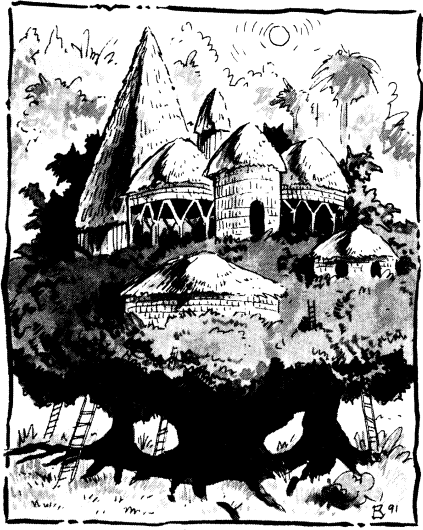
\includegraphics[width=\columnwidth]{images/gulg-1.png}
\WOTC
\end{figure}
\City{Gulg}
{13,500 (80\% humans, 7\% elves, 5\% dwarves, 3\% muls, 2\% half-elves, 2\% thri-kreen, 1\% other).}
{Agafari, copra, feathers, livestock, spices, textiles.}
{Common, Dwarven, Elven, Gulgan.}
{
	The city-state of Gulg sits inside the southern portion of the Crescent Forest, almost directly east of Tyr. Being east of the Windbreak Mountains, Gulg was spared the devastation that the Great Earthquake visited on the cities and villages to the west. That doesn't mean that life in Gulg has remained unaffected by the changes sweeping through the Tablelands. In a few significant ways, Gulg has been changed the most.

	Gulg's sorcerer-queen, Lalali-Puy (LE female champion of Rajaat stage III dragon, defiler 5/telepath 6/arch defiler 5/thrallherd 4/cerebremancer 5/Athasian dragon 2), is the absolute monarch of her realm. Her subjects consider her to be the Oba, the forest goddess. Over the centuries that she's been in power, Lalali-Puy has come to relish the worship and adoration her subjects heap upon her. In fact, though she remembers her origins as a Champion of Rajaat and a sorcerer-queen, she prefers to think of herself as the goddess her people believe her to be.

	To the Oba of Gulg, the abundance of rain---even the violent rain that accompanies a Tyr-storm---is a blessing to Athas. She has proclaimed this blessing to be a gift from the forest goddess. ``No longer will Gulg be solely concerned with the well-being of Gulg,'' the Oba declared to her people. ``Wherever the rain falls, there will the forest grow. And wherever the forest grows, the forest goddess will be there, for all the forests belong to the Oba.''

	Behind the rhetoric, Lalali-Puy actually wants to help restore the vitality of Athas. The Gulgs have always had an enlightened understanding of the interconnected nature of all life, so they've always treated the forest as a precious resource that must be maintained and not depleted. This attitude comes right from the Oba herself, which may seem strange as she is a defiler of extreme power. Since taking over Gulg, however, she has learned to temper her use of defiling magic in favor of keeping her forest healthy.

	Of course, this attitude was one of the contributing factors to the problems with Nibenay. The Nibenese saw the forest as a resource to be exploited, not a living thing that cares for its inhabitants as they care for it. Nonetheless, Lalali-Puy has made the first moves toward a peaceful existence with Nibenay, going so far as to teach the sorcerer-king how to preserve the life-giving environment of the Crescent Forest.

	The Oba's motivation isn't entirely selfless. She believes that when the forests return to Athas she will be deified by all races, just like she's been in Gulg. ``Let Nibenay and Hamanu play as sorcerer-kings,'' she has decided, ``for in the end I will be as a god to all of Athas.''
}
{
	The \emph{dagada} is the single most influential social force on Gulgs outside of the immediate family. The dagada is an extremely close-knit community that shares attributes of both clans and neighborhoods found in other societies. It is similar to a neighborhood in that it is a social organization defined first and foremost by physical proximity. It is like a clan in the role that it plays in acculturating an individual to the values of the society.

	The word dagada is used to describe both a cluster of huts and the people who live there. A dagada can contain up to 100 huts, and typically includes a number of families, though extended families may not necessarily live in the same dagada. Each dagada has a large degree of autonomy in managing its affairs as well as a degree of responsibility for all the members of the dagada. All parents have the burden of raising the young children of the dagada. Elders are responsible for educating the youths as they go. All members have a social duty to care for those who cannot provide for themselves.

	Life has always been more tolerable in Gulg than in any of the other city-states under the rule of sorcerer-kings. In some ways, life has actually gotten better for the Gulgs. The Oba's newfound crusade to restore Athas has made her more forgiving of and generous to her loyal citizens. In the spirit of cooperation, she has selected her best templars to travel the Tyr Region and spread the word of restoration. These templars have a twofold purpose. First, they help show the rest of the Tablelands how to work in harmony with nature, which Lalali-Puy hopes will hasten the reforestation of the world. Second, her templars pass along the tale that the rain is a blessing from the Oba, thereby increasing the number of people who know of and believe in Lalali-Puy.

	Except for the aid these templars have provided to Nibenay, no other city-state has thus far been targeted by the Oba's select force. Instead, the templars visit villages and oasis communities, teaching and preaching as circumstances permit. Some places have welcomed the templars, others have driven them away. Those communities that have actually experienced a Tyr-storm, for example, are quick to attack anyone who claims to be associated with their fearful properties, while those desperately in need of water invite them in.
}
{
\begin{figure*}[b!]
\centering
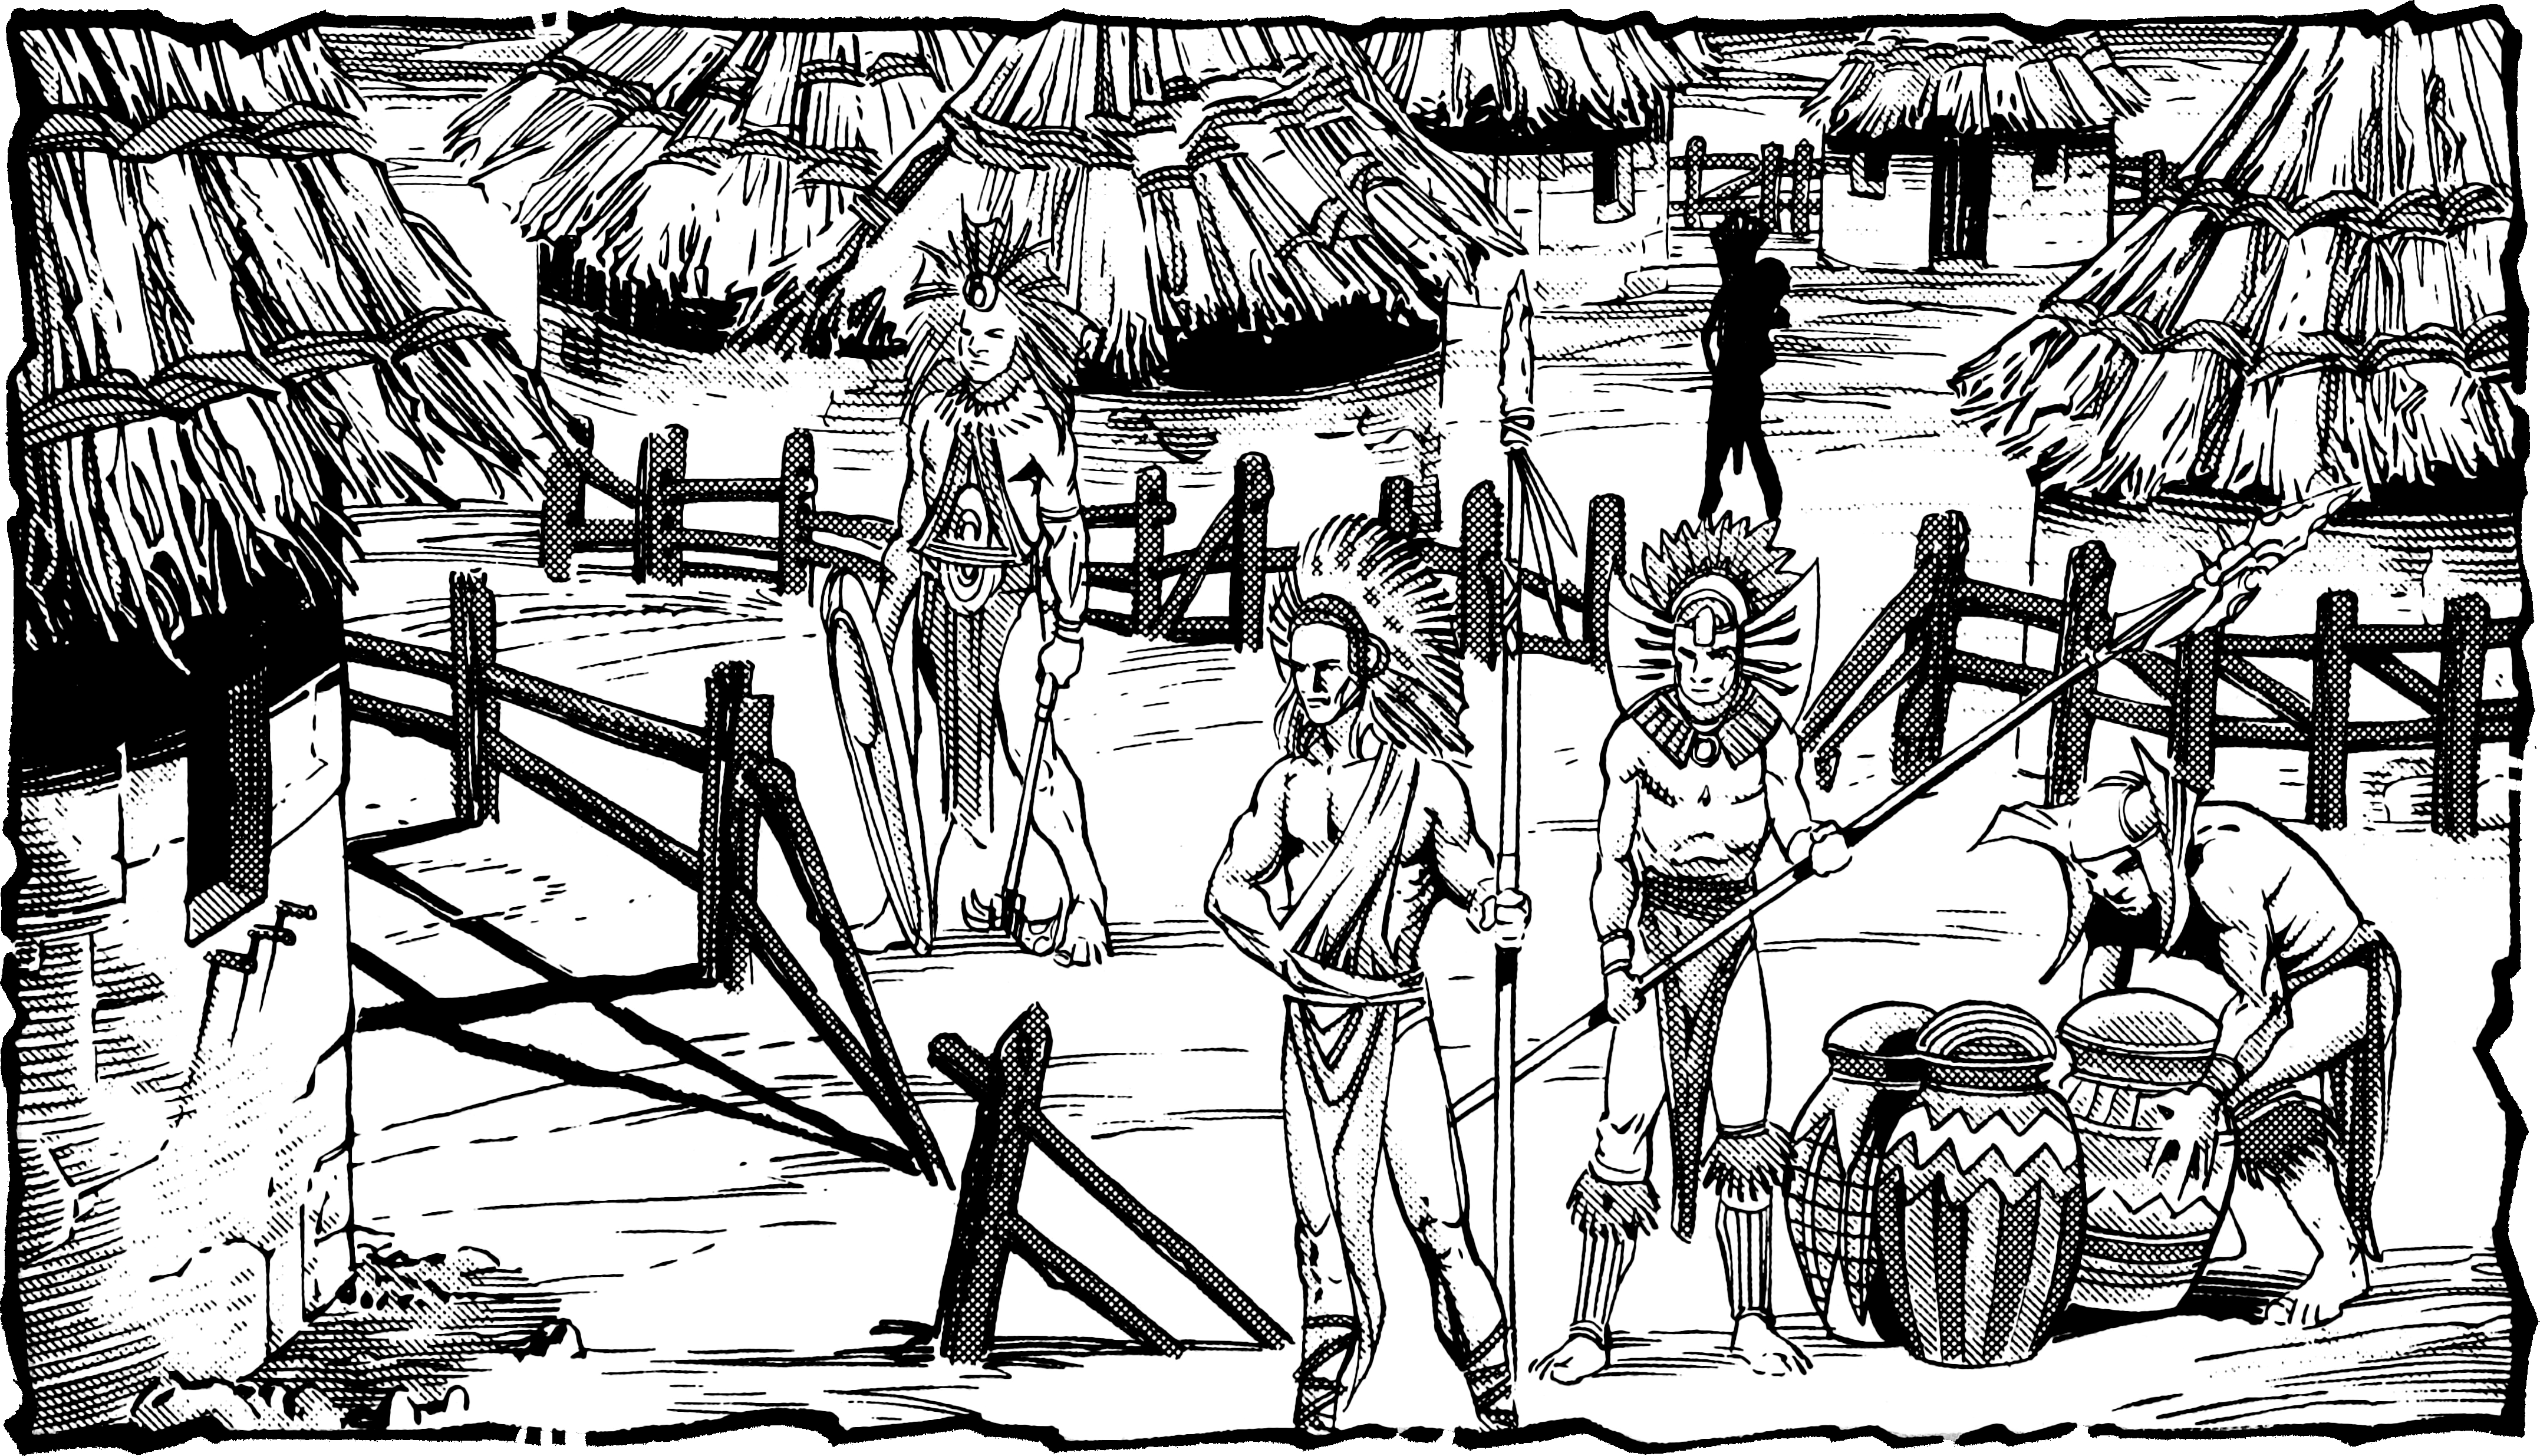
\includegraphics[width=\textwidth]{images/gulg-2.png}
\WOTC
\end{figure*}

	In many respects, Gulg is not like any of the other city-states of the Tyr Region. It's a living city, grown from vines and trees instead of constructed from brick and stone. The outer walls of the city, for example, consist of a thick hedge of thorny trees. The Oba lives in the tallest branches of a huge agafari tree, while her templars inhabit the lower branches. There are no paved or cobblestone roads leading through Gulg. Instead, forest paths and trails wind their way between the trees.

	There have been few major changes in the way Gulg is ruled. The Oba remains the owner of everything, distributing food, water, and other supplies to where they are needed most. Her templars continue to oversee the military, economic, and agricultural aspects of the community on behalf of the forest goddess. Nobility is still an earned position, not one granted by an accident of birth. The nobles hunt the forest for fresh meat, while slaves commanded by the templars gather the wild fruits, nuts, and berries that round out the dietary concerns of the community.
}
{
	\textbf{House Inika:} House Inika, the largest merchant family based in Gulg, is smaller than the typical merchant house. They specialize in small light weight goods of high value, such as spices, gemstones, and feathers from the exotic birds of the Crescent Forest. Inika maintains cordial relations with most of the other houses as it has a reputation for being nonconfrontational. Direct force is rarely used against rivals, with intrigue and economic means being the house's preferred means of strike back at rivals who try to take advantage of the house. The matriarch of the house is Andiama Inika (LN female human, rogue 14/ dune trader 5) who has ruled the house for more than two decades.

	\textbf{Judaga:} Nobility in Gulg is not granted by birth. Instead nobles must earn their position by proving they have the hunting skills necessary to provide meat for the rest of the community. There are several ways in which a citizen can become a noble. One of the most widely known ways a hunter can earn the rank of nobility is by participating in the Red Moon Hunt. During the hunt, prisoners are released unarmed into the Crescent Forest, and a thousand seconds later the hunters are sent after them. If a hunter returns with the head of the prisoners he has earned noble status, which will be bestowed upon him in a ceremony at the next High Sun. The Red Moon hunt is held on nights when the moon Ral is full and alone in the night sky.

	\textbf{The Paper Nest:} The Paper Nest is a secret society comprised of nobles favored by the Oba. The twelve to twenty-four members meet in a secret chamber in the trunk of the Sunlight Home to perform the sacred task of making paper. There is another reason for the group's existence besides making paper. Lalali-Puy attends the meetings and listens as the members debate current problems, offer advice, and present their counsel. At no other time does the autocratic Lalali-Puy allow her subjects to participate in the city's governance.

	\textbf{The Veiled Alliance:} A significant change in Gulg society concerns the Veiled Alliance of the city. Gulg's Veiled Alliance has always actively worked to restore Athas to its verdant glory, never directly opposing the will of the sorcerer-queen.

	Now that the Oba has declared her own intentions for restoring Athas, the two seem to have less to fight over. The Oba has even extended a ``peace leaf'' to the Alliance, calling for the preservers to shed the veil of secrecy and join the forest goddess's quest to save the world. The Alliance hasn't responded yet, but rumors persist that the preservers will soon come out of hiding in the forest city. The Alliance's leader, Aukash-Pad (LG male human, preserver 6/veiled one 5/earth cleric 3/psychic theurge 1), is utterly committed to restoring Athas' life force. If the Oba continues to genuinely work toward that same goal, he may be forced to join with her for the good of the world.
}
{
	\textbf{Losthome (Thorp, 60):} Losthome is a halfling community deep in the Crescent Forest. The community is less than 10 years old and was formed when the Oba of Gulg attempted to form an alliance with a halfling tribe from the Forest Ridge. An agreement was made, but shortly after the halfling warriors arrived in Gulg, their chief died. The halflings believed that the death of their chief ended the agreement and sought to return to their home, but Lalali-Puy refused to let them go and imprisoned them. Over the years since, most of the halflings have escaped into the Crescent Forest and banded together around their leader, Zivlil (N male halfling, preserver 5/kineticist 3/cerebremancer 2). The halflings maintain no permanent settlement but roam an area of the forest approximately 60 kilometers wide, in which they have a number of prepared resting areas. The halflings wish to keep their existence a secret to convince the templars of Gulg that they died in the forest. So they kill any nonhalfling who sees them.
}
{
	\textbf{The Drum Circle:} The bard's quarter in Gulg is centered around a dagada called the Drum Circle. The bards of the Gulg specialize in percussion instruments. The most skilled bard in the Drum Circle is considered to be Ken-kenku Vek (NE male half-elf, bard 12). His skills as a drummer and an assassin are legendary.

	\textbf{The Forest Arena:} The gladiator arena of Gulg is located outside the city's mopti wall in the Crescent Forest. Trees and vines intertwine with the arena to give it the appearance of growing from the forest. The floor of the arena is oval shaped, and covered with grass. A number of trees grow from the arena floor; however, none is closer than 6 meters from the arena's walls, to prevent gladiators from using them to escape.

	\textbf{The Grove of Mysteries:} Throughout the forest surrounding Gulg there are a number of forest groves called the Queen's Groves. Entrance into one of these groves without the permission of the Oba is punishable by death. The Grove of Mysteries is the largest of the Queen's Groves and is tended by the druid Extambolan (N male mul, druid 5/grove master 10).

	\textbf{Mopti Wall:} Unlike the walls of other city-states, the walls around Gulg are alive. The Mopti wall is a miles long thorn wall make of thickly packed brambleweed that surrounds the city.

	\textbf{The Seers' Dagada:} When a Gulg shows psionic potential they are sent to the Seers' dagada, where they receive instruction from experienced psions. The teachers are patient and encouraging towards the students. Even those who fail to develop enough psionic potential are not cast out, but remain part of the Seers' dagada performing physical chores for the other members.

	\textbf{Sunlight Home:} Sunlight Home is the name given to the palace of Sorcerer-Queen, Lalali-Puy. Located in the tallest branches of a massive agafari tree, Sunlight Home towers over the rest of the city. Lalali-Puy's palace is rumored to contain dungeons and secret passages that have been carved into the trunk of the massive tree.
}
{
	\item Ngeli is a small boy of ten years old. While gathering cloves in the forest he was attacked and dragged off by a sloth. His parents are distraught and want to see a rescue attempt made to recover their boy, but the ambo of their dagada ruled that the boy was taken by the nature spirits and should be given up to his fate. Ngeli's parents turn to outsiders, the PCs, to secretly bring back their boy.
	\item The berry harvest has finished for the year. The berries had a strange brownish tint, but seemed fine to the taste. But those who have eaten too much of the berries have been having strange reactions. Some exhibit strange new psionic powers, others become sick and die, and some fall into a suggestive state and will do nothing but what others tell them to do.
	\item Alexia Vordon trades for spices with Gulg. She feels that her house trades at a disadvantage by being forced to deal with the templars. If she can make contact with a member of the spice gathers she is convinced that she will have a better understanding of how good the year's harvest has been and be in a better position to negotiate with the templars. Alexia hires the PCs to sneak her into the city and help her try to befriend someone from the spice gatherers dagada.
	\item Rumors in the neighborhood have begun that a teenage girl is really a witch. The wild rumors began when the girl started wearing a veil that covers her face leaving only her eyes showing. Many hot-headed, superstitious members of her dagada are contemplating drastic actions against the girl. The PCs will have to find some way to stop these rumors. The truth is that the girl has experienced her first heavy case of acne. Unsure of what is really happening to her, and fearful that others will reject her because of her affliction, she hides behind the veil, refusing to remove the veil and revealing her affliction to anyone.
	\item The PCs are invited on a hunt with a group of nobles from Gulg. The nobles seek to test the PCs hunting skills. They hang back letting the PCs take the lead, while hunting a dangerous beast, such as a klar.
	\item The templar, Kampala, has a feylaar as his fetish. When visiting a small client village, he summons the totem spirit, only to have it break from his control and go on a rampage.
}